\documentclass[tikz,border=0pt]{standalone}
\usepackage{xcolor}
% Palette: Sam_Comm_final.png by eye (as Pursuer's art.py), and Gatecrasher's own.
\definecolor{ink}{HTML}{3B2340}
\definecolor{sky}{HTML}{EFC46A}
\definecolor{skyhi}{HTML}{F5DA92}
\definecolor{skylow}{HTML}{E9B060}
\definecolor{cloud}{HTML}{F2D58A}
\definecolor{wallA}{HTML}{E88A73}
\definecolor{wallB}{HTML}{EE9F7E}
\definecolor{wallC}{HTML}{E47A7E}
\definecolor{wallD}{HTML}{F0B07E}
\definecolor{wallE}{HTML}{D9765F}
\definecolor{wallF}{HTML}{E99A8A}
\definecolor{greenA}{HTML}{8DBB7E}
\definecolor{greenB}{HTML}{6FA77A}
\definecolor{greenC}{HTML}{A9C97F}
\definecolor{greenD}{HTML}{5E9C6A}
\definecolor{window}{HTML}{F6E7A0}
\definecolor{windark}{HTML}{8C5A64}
\definecolor{metal}{HTML}{8D9A93}
\definecolor{metaldark}{HTML}{5E6B66}
\definecolor{wood}{HTML}{B9835A}
\definecolor{paving}{HTML}{E2BD8C}
\definecolor{ground}{HTML}{D3A77D}
\definecolor{stone}{HTML}{E7C9A0}
\definecolor{paper}{HTML}{F6E7C4}
\definecolor{cardboard}{HTML}{C9A06A}
\definecolor{cardboarddark}{HTML}{A47C4C}
\definecolor{red}{HTML}{B3262E}
\definecolor{eyewhite}{HTML}{FBF4E4}
\definecolor{skin}{HTML}{E8B07C}
\definecolor{skinB}{HTML}{C98B5E}
\definecolor{skinC}{HTML}{F2C9A0}
\definecolor{hairdark}{HTML}{2A1E33}
\definecolor{hairred}{HTML}{A8553A}
\definecolor{leather}{HTML}{33293D}
\definecolor{chrome}{HTML}{C9D3CF}
\definecolor{chromedark}{HTML}{7F8C88}
\definecolor{glass}{HTML}{A9D4CB}
\definecolor{lamp}{HTML}{FFE6A3}
\definecolor{smoke}{HTML}{E8D3AE}
\definecolor{shingle}{HTML}{C9604F}
\definecolor{gold}{HTML}{F2B53A}
\definecolor{portalblue}{HTML}{2FA8E8}
\definecolor{portalbluehi}{HTML}{A6DDF5}
\definecolor{portalorange}{HTML}{F2812E}
\definecolor{portalorangehi}{HTML}{F9C891}
\definecolor{olive}{HTML}{7A8450}
\definecolor{olivedark}{HTML}{5C6539}
\definecolor{khaki}{HTML}{C2A66E}
\definecolor{khakidark}{HTML}{9E8350}
\definecolor{mule}{HTML}{9A6A44}
\definecolor{muledark}{HTML}{6B4730}
\definecolor{mulelight}{HTML}{C99A6E}
\definecolor{bandana}{HTML}{C8343A}
\definecolor{suit}{HTML}{56704F}
\definecolor{camoA}{HTML}{8DA867}
\definecolor{camoB}{HTML}{3B5240}
\definecolor{lens}{HTML}{8EF0C6}
\definecolor{lenshi}{HTML}{E2FFF2}
\definecolor{sea}{HTML}{5FB3B0}
\definecolor{seahi}{HTML}{8FCFC0}
\definecolor{seadark}{HTML}{3F8F92}
\definecolor{concrete}{HTML}{E6C29A}
\definecolor{concretedark}{HTML}{C9A07A}
\definecolor{heli}{HTML}{4F8F86}
\definecolor{helidark}{HTML}{3A6C66}
\definecolor{duskA}{HTML}{7A5272}
\definecolor{duskB}{HTML}{B06A78}
\definecolor{duskC}{HTML}{DE8E72}
\definecolor{dirt}{HTML}{C08A68}
\definecolor{dirtdark}{HTML}{A87256}
\definecolor{beam}{HTML}{FFF3BE}
\definecolor{sunA}{HTML}{F3B86A}
\definecolor{sunB}{HTML}{EE9268}
\definecolor{sunC}{HTML}{E57766}
\definecolor{sundisc}{HTML}{FBE3A0}
\definecolor{seadusk}{HTML}{6F9E9C}
\definecolor{balloon}{HTML}{F8F0DE}
\definecolor{hay}{HTML}{E9C46A}
\definecolor{haydark}{HTML}{C99B45}
\definecolor{barn}{HTML}{C9604F}
\definecolor{trim}{HTML}{F6E7C4}
\begin{document}
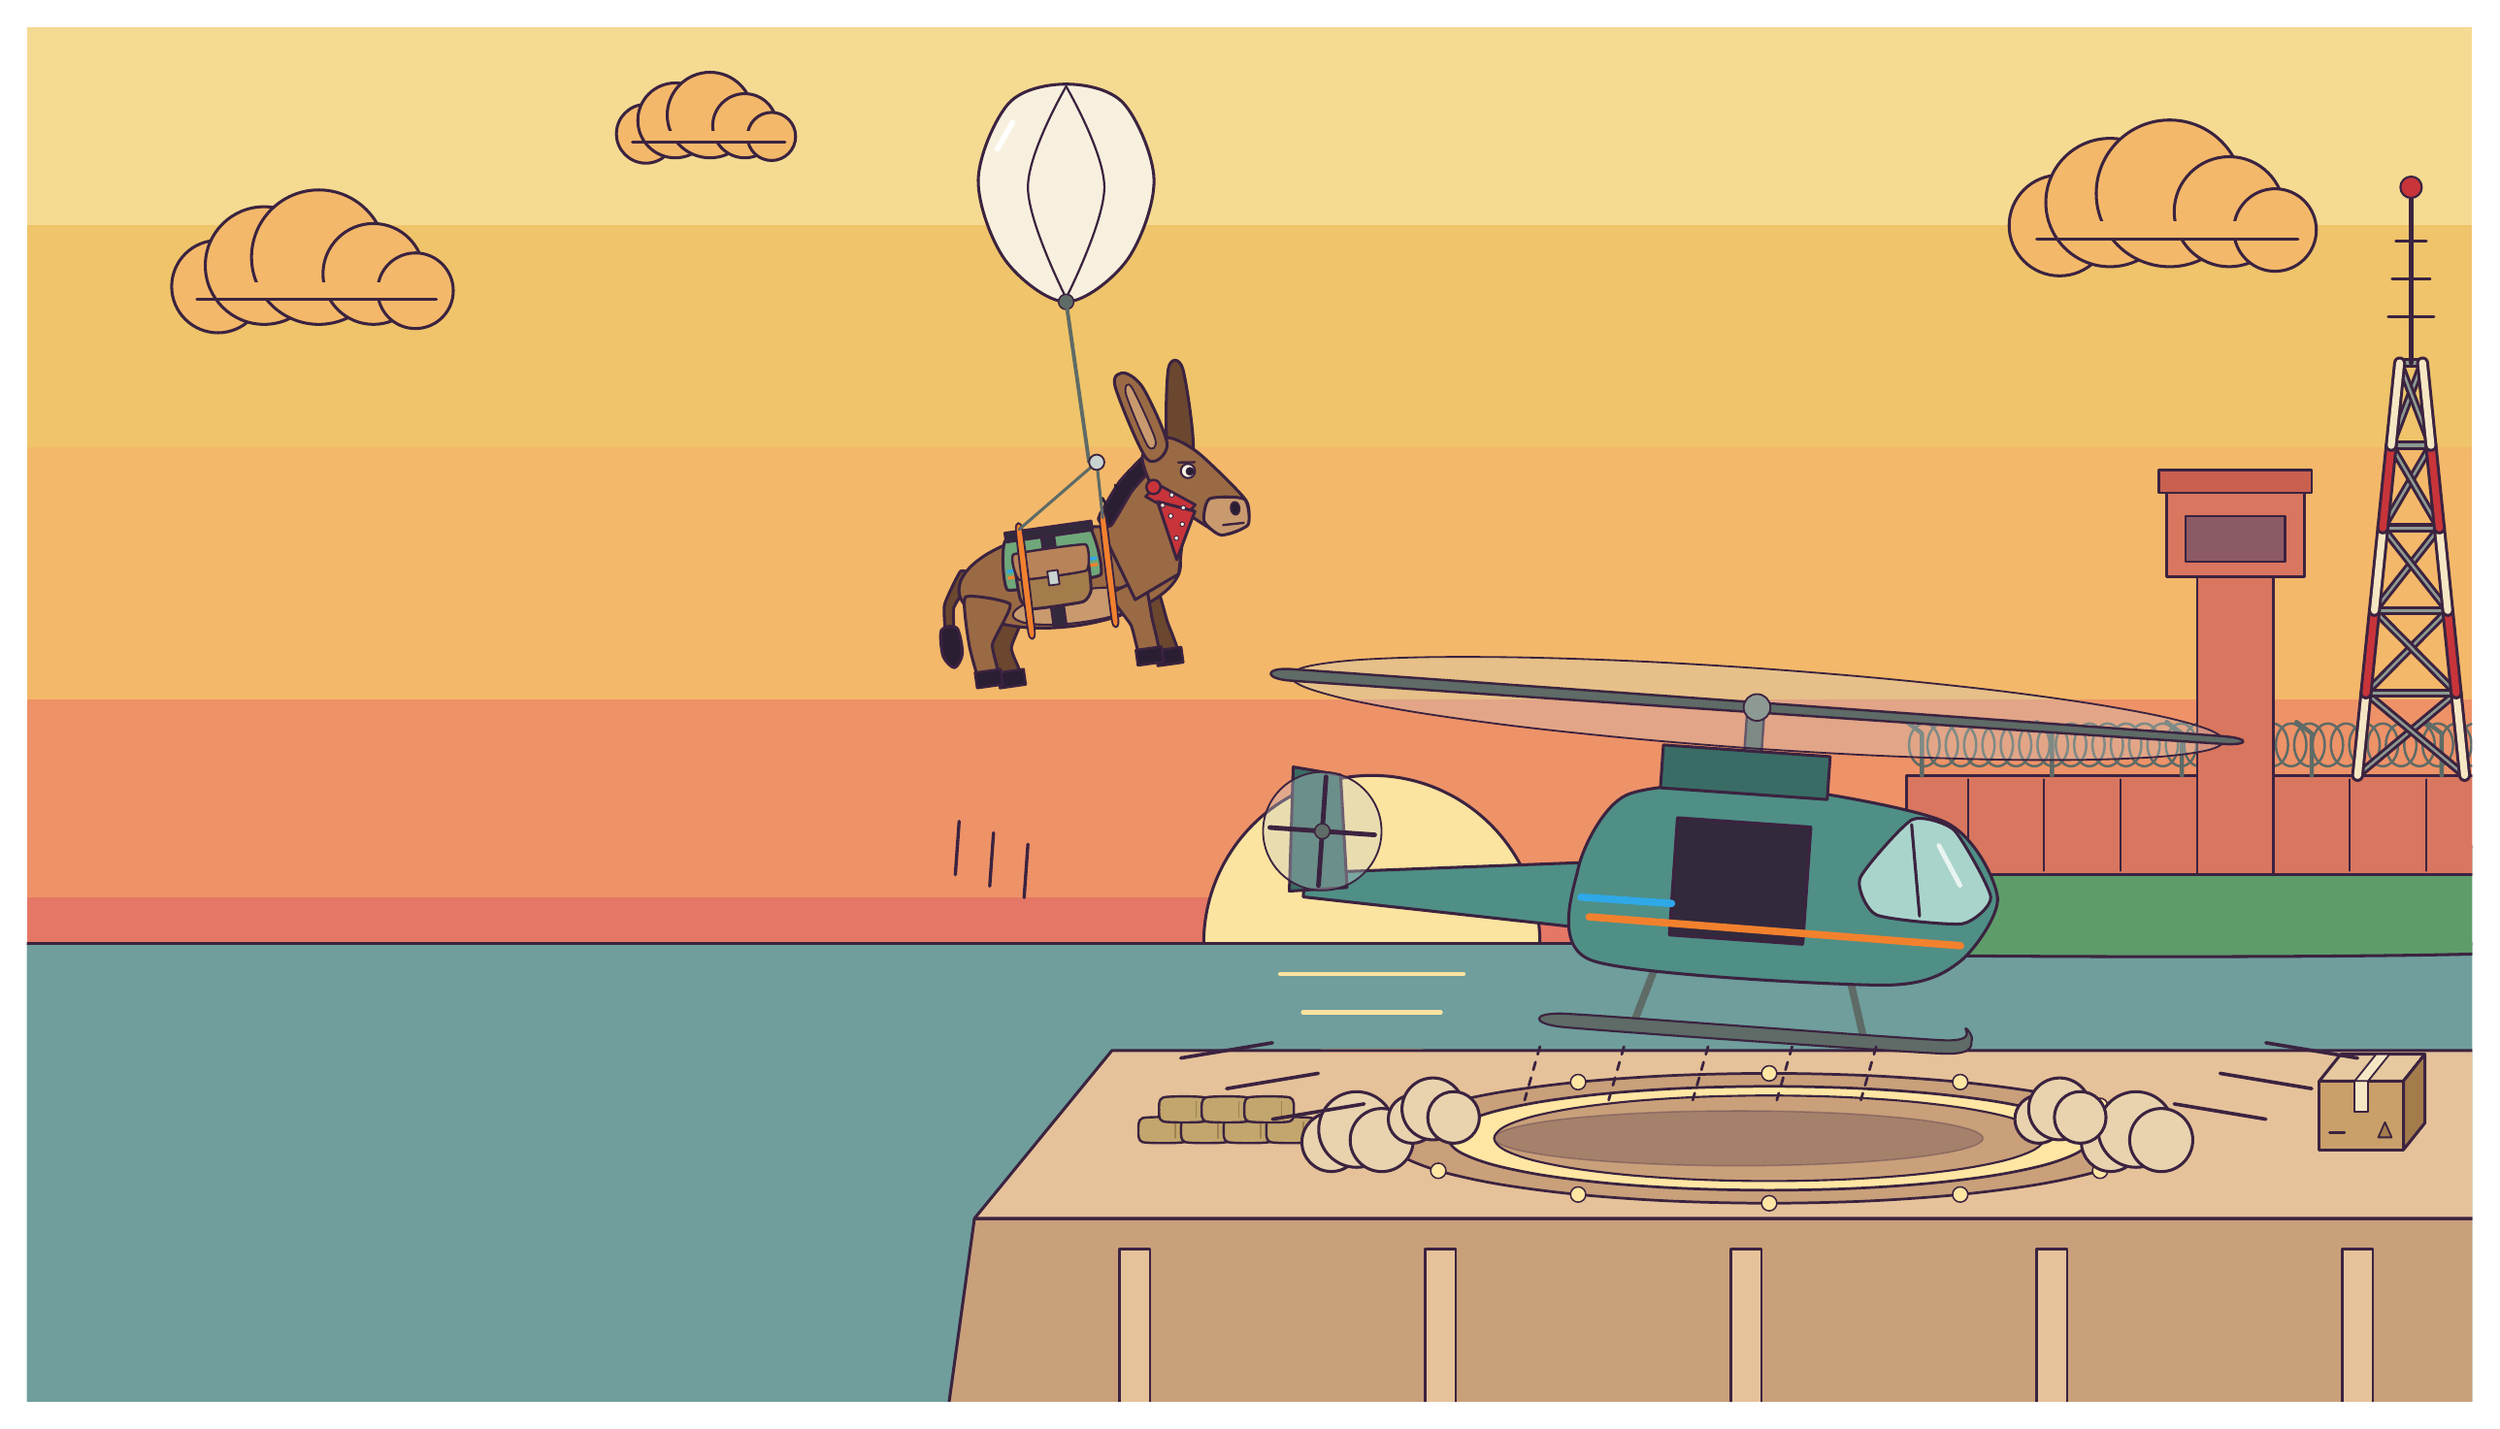
\begin{tikzpicture}
\useasboundingbox (0,0) rectangle (32,18);
\clip (0,0) rectangle (32,18);
\fill[sunC] (0,0) rectangle (32,18);
\fill[sunB] (0,6.6) rectangle (32,18);
\fill[sunA] (0,9.2) rectangle (32,18);
\fill[sky] (0,12.5) rectangle (32,18);
\fill[skyhi] (0,15.4) rectangle (32,18);
\filldraw[draw=ink, line width=1.1pt, line join=round, fill=sunA] (2.5,14.6) circle (0.605);
\filldraw[draw=ink, line width=1.1pt, line join=round, fill=sunA] (3.105,14.875) circle (0.77);
\filldraw[draw=ink, line width=1.1pt, line join=round, fill=sunA] (3.82,14.985) circle (0.88);
\filldraw[draw=ink, line width=1.1pt, line join=round, fill=sunA] (4.535,14.765) circle (0.66);
\filldraw[draw=ink, line width=1.1pt, line join=round, fill=sunA] (5.085,14.545) circle (0.495);
\fill[sunA] (2.5,14.435) rectangle (5.085,14.655);
\draw[ink, line width=1.1pt, line cap=round, line join=round] (2.225,14.435) -- (5.36,14.435);
\filldraw[draw=ink, line width=1.1pt, line join=round, fill=sunA] (8.1,16.6) circle (0.385);
\filldraw[draw=ink, line width=1.1pt, line join=round, fill=sunA] (8.485,16.775) circle (0.49);
\filldraw[draw=ink, line width=1.1pt, line join=round, fill=sunA] (8.94,16.845) circle (0.56);
\filldraw[draw=ink, line width=1.1pt, line join=round, fill=sunA] (9.395,16.705) circle (0.42);
\filldraw[draw=ink, line width=1.1pt, line join=round, fill=sunA] (9.745,16.565) circle (0.315);
\fill[sunA] (8.1,16.495) rectangle (9.745,16.635);
\draw[ink, line width=1.1pt, line cap=round, line join=round] (7.925,16.495) -- (9.92,16.495);
\filldraw[draw=ink, line width=1.1pt, line join=round, fill=sunA] (26.6,15.4) circle (0.66);
\filldraw[draw=ink, line width=1.1pt, line join=round, fill=sunA] (27.26,15.7) circle (0.84);
\filldraw[draw=ink, line width=1.1pt, line join=round, fill=sunA] (28.04,15.82) circle (0.96);
\filldraw[draw=ink, line width=1.1pt, line join=round, fill=sunA] (28.82,15.58) circle (0.72);
\filldraw[draw=ink, line width=1.1pt, line join=round, fill=sunA] (29.42,15.34) circle (0.54);
\fill[sunA] (26.6,15.22) rectangle (29.42,15.46);
\draw[ink, line width=1.1pt, line cap=round, line join=round] (26.3,15.22) -- (29.72,15.22);
\filldraw[draw=ink, line width=1.1pt, line join=round, fill=sundisc] (17.6,6) circle (2.2);
\filldraw[draw=ink, line width=1.1pt, fill=seadusk] (-0.5,-0.5) rectangle (32.5,6);
\draw[sundisc, line width=1.6pt, line cap=round, line join=round] (16.4,5.6) -- (18.8,5.6);
\draw[sundisc, line width=1.6pt, line cap=round, line join=round] (16.7,5.1) -- (18.5,5.1);
\draw[sundisc, line width=1.6pt, line cap=round, line join=round] (16.95,4.6) -- (18.25,4.6);
\draw[sundisc, line width=1.6pt, line cap=round, line join=round] (17.2,4.1) -- (18,4.1);
\filldraw[draw=ink, line width=1.1pt, line join=round, fill=greenD] plot[smooth cycle, tension=0.3] coordinates {(22.5,5.9) (24.5,6.9) (28,7.3) (32.8,7.2) (32.8,5.9)};
\filldraw[draw=ink, line width=0.99pt, line join=round, fill=wallE] (24.6,6.9) -- (32.6,6.9) -- (32.6,8.2) -- (24.6,8.2) -- cycle;
\draw[ink, line width=0.7pt, line cap=round, line join=round] (25.4,6.95) -- (25.4,8.15);
\draw[ink, line width=0.7pt, line cap=round, line join=round] (26.4,6.95) -- (26.4,8.15);
\draw[ink, line width=0.7pt, line cap=round, line join=round] (27.4,6.95) -- (27.4,8.15);
\draw[ink, line width=0.7pt, line cap=round, line join=round] (28.4,6.95) -- (28.4,8.15);
\draw[ink, line width=0.7pt, line cap=round, line join=round] (29.4,6.95) -- (29.4,8.15);
\draw[ink, line width=0.7pt, line cap=round, line join=round] (30.4,6.95) -- (30.4,8.15);
\draw[ink, line width=0.7pt, line cap=round, line join=round] (31.4,6.95) -- (31.4,8.15);
\draw[ink, line width=0.7pt, line cap=round, line join=round] (32.4,6.95) -- (32.4,8.15);
\draw[metaldark, line width=1.6pt, line cap=round, line join=round] (24.8,8.2) -- (24.8,8.75) -- (24.6,8.9);
\draw[metaldark, line width=1.6pt, line cap=round, line join=round] (26.5,8.2) -- (26.5,8.75) -- (26.3,8.9);
\draw[metaldark, line width=1.6pt, line cap=round, line join=round] (28.2,8.2) -- (28.2,8.75) -- (28,8.9);
\draw[metaldark, line width=1.6pt, line cap=round, line join=round] (29.9,8.2) -- (29.9,8.75) -- (29.7,8.9);
\draw[metaldark, line width=1.6pt, line cap=round, line join=round] (31.6,8.2) -- (31.6,8.75) -- (31.4,8.9);
\draw[metaldark, line width=0.9pt] (24.83,8.6) ellipse (0.2 and 0.28);
\draw[metaldark, line width=0.9pt] (25.07,8.6) ellipse (0.2 and 0.28);
\draw[metaldark, line width=0.9pt] (25.31,8.6) ellipse (0.2 and 0.28);
\draw[metaldark, line width=0.9pt] (25.55,8.6) ellipse (0.2 and 0.28);
\draw[metaldark, line width=0.9pt] (25.79,8.6) ellipse (0.2 and 0.28);
\draw[metaldark, line width=0.9pt] (26.03,8.6) ellipse (0.2 and 0.28);
\draw[metaldark, line width=0.9pt] (26.27,8.6) ellipse (0.2 and 0.28);
\draw[metaldark, line width=0.9pt] (26.51,8.6) ellipse (0.2 and 0.28);
\draw[metaldark, line width=0.9pt] (26.75,8.6) ellipse (0.2 and 0.28);
\draw[metaldark, line width=0.9pt] (26.99,8.6) ellipse (0.2 and 0.28);
\draw[metaldark, line width=0.9pt] (27.23,8.6) ellipse (0.2 and 0.28);
\draw[metaldark, line width=0.9pt] (27.47,8.6) ellipse (0.2 and 0.28);
\draw[metaldark, line width=0.9pt] (27.71,8.6) ellipse (0.2 and 0.28);
\draw[metaldark, line width=0.9pt] (27.95,8.6) ellipse (0.2 and 0.28);
\draw[metaldark, line width=0.9pt] (28.19,8.6) ellipse (0.2 and 0.28);
\draw[metaldark, line width=0.9pt] (28.43,8.6) ellipse (0.2 and 0.28);
\draw[metaldark, line width=0.9pt] (28.67,8.6) ellipse (0.2 and 0.28);
\draw[metaldark, line width=0.9pt] (28.91,8.6) ellipse (0.2 and 0.28);
\draw[metaldark, line width=0.9pt] (29.15,8.6) ellipse (0.2 and 0.28);
\draw[metaldark, line width=0.9pt] (29.39,8.6) ellipse (0.2 and 0.28);
\draw[metaldark, line width=0.9pt] (29.63,8.6) ellipse (0.2 and 0.28);
\draw[metaldark, line width=0.9pt] (29.87,8.6) ellipse (0.2 and 0.28);
\draw[metaldark, line width=0.9pt] (30.11,8.6) ellipse (0.2 and 0.28);
\draw[metaldark, line width=0.9pt] (30.35,8.6) ellipse (0.2 and 0.28);
\draw[metaldark, line width=0.9pt] (30.59,8.6) ellipse (0.2 and 0.28);
\draw[metaldark, line width=0.9pt] (30.83,8.6) ellipse (0.2 and 0.28);
\draw[metaldark, line width=0.9pt] (31.07,8.6) ellipse (0.2 and 0.28);
\draw[metaldark, line width=0.9pt] (31.31,8.6) ellipse (0.2 and 0.28);
\draw[metaldark, line width=0.9pt] (31.55,8.6) ellipse (0.2 and 0.28);
\draw[metaldark, line width=0.9pt] (31.79,8.6) ellipse (0.2 and 0.28);
\draw[metaldark, line width=0.9pt] (32.03,8.6) ellipse (0.2 and 0.28);
\draw[metaldark, line width=0.9pt] (32.27,8.6) ellipse (0.2 and 0.28);
\draw[metaldark, line width=0.9pt] (32.51,8.6) ellipse (0.2 and 0.28);
\filldraw[draw=ink, line width=0.99pt, line join=round, fill=wallE] (28.4,6.9) -- (29.4,6.9) -- (29.4,10.8) -- (28.4,10.8) -- cycle;
\filldraw[draw=ink, line width=0.99pt, line join=round, fill=wallE] (28,10.8) -- (29.8,10.8) -- (29.8,11.9) -- (28,11.9) -- cycle;
\filldraw[draw=ink, line width=0.77pt, line join=round, fill=windark] (28.25,11) -- (29.55,11) -- (29.55,11.6) -- (28.25,11.6) -- cycle;
\filldraw[draw=ink, line width=0.88pt, line join=round, fill=shingle] (27.9,11.9) -- (29.9,11.9) -- (29.9,12.2) -- (27.9,12.2) -- cycle;
\draw[ink, line width=3.1pt, line cap=round, line join=round] (30.5,8.2) -- (31.79,9.28);
\draw[metal, line width=0.9pt, line cap=round, line join=round] (30.5,8.2) -- (31.79,9.28);
\draw[ink, line width=3.1pt, line cap=round, line join=round] (31.9,8.2) -- (30.61,9.28);
\draw[metal, line width=0.9pt, line cap=round, line join=round] (31.9,8.2) -- (30.61,9.28);
\draw[ink, line width=3.4pt, line cap=round, line join=round] (30.61,9.28) -- (31.79,9.28);
\draw[metal, line width=1.2pt, line cap=round, line join=round] (30.61,9.28) -- (31.79,9.28);
\draw[ink, line width=3.1pt, line cap=round, line join=round] (30.61,9.28) -- (31.68,10.36);
\draw[metal, line width=0.9pt, line cap=round, line join=round] (30.61,9.28) -- (31.68,10.36);
\draw[ink, line width=3.1pt, line cap=round, line join=round] (31.79,9.28) -- (30.72,10.36);
\draw[metal, line width=0.9pt, line cap=round, line join=round] (31.79,9.28) -- (30.72,10.36);
\draw[ink, line width=3.4pt, line cap=round, line join=round] (30.72,10.36) -- (31.68,10.36);
\draw[metal, line width=1.2pt, line cap=round, line join=round] (30.72,10.36) -- (31.68,10.36);
\draw[ink, line width=3.1pt, line cap=round, line join=round] (30.72,10.36) -- (31.57,11.44);
\draw[metal, line width=0.9pt, line cap=round, line join=round] (30.72,10.36) -- (31.57,11.44);
\draw[ink, line width=3.1pt, line cap=round, line join=round] (31.68,10.36) -- (30.83,11.44);
\draw[metal, line width=0.9pt, line cap=round, line join=round] (31.68,10.36) -- (30.83,11.44);
\draw[ink, line width=3.4pt, line cap=round, line join=round] (30.83,11.44) -- (31.57,11.44);
\draw[metal, line width=1.2pt, line cap=round, line join=round] (30.83,11.44) -- (31.57,11.44);
\draw[ink, line width=3.1pt, line cap=round, line join=round] (30.83,11.44) -- (31.46,12.52);
\draw[metal, line width=0.9pt, line cap=round, line join=round] (30.83,11.44) -- (31.46,12.52);
\draw[ink, line width=3.1pt, line cap=round, line join=round] (31.57,11.44) -- (30.94,12.52);
\draw[metal, line width=0.9pt, line cap=round, line join=round] (31.57,11.44) -- (30.94,12.52);
\draw[ink, line width=3.4pt, line cap=round, line join=round] (30.94,12.52) -- (31.46,12.52);
\draw[metal, line width=1.2pt, line cap=round, line join=round] (30.94,12.52) -- (31.46,12.52);
\draw[ink, line width=3.1pt, line cap=round, line join=round] (30.94,12.52) -- (31.35,13.6);
\draw[metal, line width=0.9pt, line cap=round, line join=round] (30.94,12.52) -- (31.35,13.6);
\draw[ink, line width=3.1pt, line cap=round, line join=round] (31.46,12.52) -- (31.05,13.6);
\draw[metal, line width=0.9pt, line cap=round, line join=round] (31.46,12.52) -- (31.05,13.6);
\draw[ink, line width=3.4pt, line cap=round, line join=round] (31.05,13.6) -- (31.35,13.6);
\draw[metal, line width=1.2pt, line cap=round, line join=round] (31.05,13.6) -- (31.35,13.6);
\draw[ink, line width=4.8pt, line cap=round, line join=round] (30.5,8.2) -- (30.61,9.28);
\draw[paper, line width=2.6pt, line cap=round, line join=round] (30.5,8.2) -- (30.61,9.28);
\draw[ink, line width=4.8pt, line cap=round, line join=round] (30.61,9.28) -- (30.72,10.36);
\draw[bandana, line width=2.6pt, line cap=round, line join=round] (30.61,9.28) -- (30.72,10.36);
\draw[ink, line width=4.8pt, line cap=round, line join=round] (30.72,10.36) -- (30.83,11.44);
\draw[paper, line width=2.6pt, line cap=round, line join=round] (30.72,10.36) -- (30.83,11.44);
\draw[ink, line width=4.8pt, line cap=round, line join=round] (30.83,11.44) -- (30.94,12.52);
\draw[bandana, line width=2.6pt, line cap=round, line join=round] (30.83,11.44) -- (30.94,12.52);
\draw[ink, line width=4.8pt, line cap=round, line join=round] (30.94,12.52) -- (31.05,13.6);
\draw[paper, line width=2.6pt, line cap=round, line join=round] (30.94,12.52) -- (31.05,13.6);
\draw[ink, line width=4.8pt, line cap=round, line join=round] (31.9,8.2) -- (31.79,9.28);
\draw[paper, line width=2.6pt, line cap=round, line join=round] (31.9,8.2) -- (31.79,9.28);
\draw[ink, line width=4.8pt, line cap=round, line join=round] (31.79,9.28) -- (31.68,10.36);
\draw[bandana, line width=2.6pt, line cap=round, line join=round] (31.79,9.28) -- (31.68,10.36);
\draw[ink, line width=4.8pt, line cap=round, line join=round] (31.68,10.36) -- (31.57,11.44);
\draw[paper, line width=2.6pt, line cap=round, line join=round] (31.68,10.36) -- (31.57,11.44);
\draw[ink, line width=4.8pt, line cap=round, line join=round] (31.57,11.44) -- (31.46,12.52);
\draw[bandana, line width=2.6pt, line cap=round, line join=round] (31.57,11.44) -- (31.46,12.52);
\draw[ink, line width=4.8pt, line cap=round, line join=round] (31.46,12.52) -- (31.35,13.6);
\draw[paper, line width=2.6pt, line cap=round, line join=round] (31.46,12.52) -- (31.35,13.6);
\draw[ink, line width=1.6pt, line cap=round, line join=round] (31.2,13.6) -- (31.2,15.8);
\draw[ink, line width=1pt, line cap=round, line join=round] (30.9,14.2) -- (31.5,14.2);
\draw[ink, line width=1pt, line cap=round, line join=round] (30.95,14.7) -- (31.45,14.7);
\draw[ink, line width=1pt, line cap=round, line join=round] (31,15.2) -- (31.4,15.2);
\filldraw[draw=ink, line width=0.77pt, line join=round, fill=bandana] (31.2,15.9) circle (0.14);
\filldraw[draw=ink, line width=1.1pt, line join=round, fill=concretedark] (12,-0.5) -- (32.6,-0.5) -- (32.6,2.4) -- (12.4,2.4) -- cycle;
\filldraw[draw=ink, line width=0.88pt, line join=round, fill=concrete] (14.3,-0.5) -- (14.7,-0.5) -- (14.7,2) -- (14.3,2) -- cycle;
\filldraw[draw=ink, line width=0.88pt, line join=round, fill=concrete] (18.3,-0.5) -- (18.7,-0.5) -- (18.7,2) -- (18.3,2) -- cycle;
\filldraw[draw=ink, line width=0.88pt, line join=round, fill=concrete] (22.3,-0.5) -- (22.7,-0.5) -- (22.7,2) -- (22.3,2) -- cycle;
\filldraw[draw=ink, line width=0.88pt, line join=round, fill=concrete] (26.3,-0.5) -- (26.7,-0.5) -- (26.7,2) -- (26.3,2) -- cycle;
\filldraw[draw=ink, line width=0.88pt, line join=round, fill=concrete] (30.3,-0.5) -- (30.7,-0.5) -- (30.7,2) -- (30.3,2) -- cycle;
\filldraw[draw=ink, line width=1.1pt, line join=round, fill=concrete] (12.4,2.4) -- (32.6,2.4) -- (32.6,4.6) -- (14.2,4.6) -- cycle;
\filldraw[draw=ink, line width=0.99pt, line join=round, fill=concretedark] plot[smooth cycle, tension=0.55] coordinates {(27.8,3.45) (27.63,3.67) (27.13,3.875) (26.336,4.051) (25.3,4.186) (24.094,4.271) (22.8,4.3) (21.506,4.271) (20.3,4.186) (19.264,4.051) (18.47,3.875) (17.97,3.67) (17.8,3.45) (17.97,3.23) (18.47,3.025) (19.264,2.849) (20.3,2.714) (21.506,2.629) (22.8,2.6) (24.094,2.629) (25.3,2.714) (26.336,2.849) (27.13,3.025) (27.63,3.23)};
\filldraw[draw=ink, line width=0.99pt, line join=round, fill=lamp] plot[smooth cycle, tension=0.55] coordinates {(27,3.45) (26.857,3.626) (26.437,3.79) (25.77,3.931) (24.9,4.039) (23.887,4.107) (22.8,4.13) (21.713,4.107) (20.7,4.039) (19.83,3.931) (19.163,3.79) (18.743,3.626) (18.6,3.45) (18.743,3.274) (19.163,3.11) (19.83,2.969) (20.7,2.861) (21.713,2.793) (22.8,2.77) (23.887,2.793) (24.9,2.861) (25.77,2.969) (26.437,3.11) (26.857,3.274)};
\filldraw[draw=ink, line width=0.77pt, line join=round, fill=concretedark] plot[smooth cycle, tension=0.55] coordinates {(26.4,3.45) (26.277,3.595) (25.918,3.73) (25.346,3.846) (24.6,3.935) (23.732,3.991) (22.8,4.01) (21.868,3.991) (21,3.935) (20.254,3.846) (19.682,3.73) (19.323,3.595) (19.2,3.45) (19.323,3.305) (19.682,3.17) (20.254,3.054) (21,2.965) (21.868,2.909) (22.8,2.89) (23.732,2.909) (24.6,2.965) (25.346,3.054) (25.918,3.17) (26.277,3.305)};
\filldraw[draw=ink, line width=0.55pt, line join=round, fill=lamp] (27.8,3.45) circle (0.1);
\filldraw[draw=ink, line width=0.55pt, line join=round, fill=lamp] (27.13,3.875) circle (0.1);
\filldraw[draw=ink, line width=0.55pt, line join=round, fill=lamp] (25.3,4.186) circle (0.1);
\filldraw[draw=ink, line width=0.55pt, line join=round, fill=lamp] (22.8,4.3) circle (0.1);
\filldraw[draw=ink, line width=0.55pt, line join=round, fill=lamp] (20.3,4.186) circle (0.1);
\filldraw[draw=ink, line width=0.55pt, line join=round, fill=lamp] (18.47,3.875) circle (0.1);
\filldraw[draw=ink, line width=0.55pt, line join=round, fill=lamp] (17.8,3.45) circle (0.1);
\filldraw[draw=ink, line width=0.55pt, line join=round, fill=lamp] (18.47,3.025) circle (0.1);
\filldraw[draw=ink, line width=0.55pt, line join=round, fill=lamp] (20.3,2.714) circle (0.1);
\filldraw[draw=ink, line width=0.55pt, line join=round, fill=lamp] (22.8,2.6) circle (0.1);
\filldraw[draw=ink, line width=0.55pt, line join=round, fill=lamp] (25.3,2.714) circle (0.1);
\filldraw[draw=ink, line width=0.55pt, line join=round, fill=lamp] (27.13,3.025) circle (0.1);
\filldraw[draw=ink, line width=0.55pt, line join=round, fill=ink, fill opacity=0.25, draw opacity=0.3] plot[smooth cycle, tension=0.55] coordinates {(25.6,3.45) (25.491,3.543) (25.171,3.63) (24.663,3.705) (24,3.762) (23.228,3.798) (22.4,3.81) (21.572,3.798) (20.8,3.762) (20.137,3.705) (19.629,3.63) (19.309,3.543) (19.2,3.45) (19.309,3.357) (19.629,3.27) (20.137,3.195) (20.8,3.138) (21.572,3.102) (22.4,3.09) (23.228,3.102) (24,3.138) (24.663,3.195) (25.171,3.27) (25.491,3.357)};
\filldraw[draw=ink, line width=0.88pt, line join=round, fill=khaki] plot[smooth cycle, tension=0.4] coordinates {(14.6,3.4) (15.14,3.4) (15.194,3.553) (15.14,3.715) (14.6,3.715) (14.546,3.553)};
\draw[khakidark, line width=0.6pt, line cap=round, line join=round] (15.032,3.454) -- (15.032,3.661);
\filldraw[draw=ink, line width=0.88pt, line join=round, fill=khaki] plot[smooth cycle, tension=0.4] coordinates {(15.158,3.4) (15.698,3.4) (15.752,3.553) (15.698,3.715) (15.158,3.715) (15.104,3.553)};
\draw[khakidark, line width=0.6pt, line cap=round, line join=round] (15.59,3.454) -- (15.59,3.661);
\filldraw[draw=ink, line width=0.88pt, line join=round, fill=khaki] plot[smooth cycle, tension=0.4] coordinates {(15.716,3.4) (16.256,3.4) (16.31,3.553) (16.256,3.715) (15.716,3.715) (15.662,3.553)};
\draw[khakidark, line width=0.6pt, line cap=round, line join=round] (16.148,3.454) -- (16.148,3.661);
\filldraw[draw=ink, line width=0.88pt, line join=round, fill=khaki] plot[smooth cycle, tension=0.4] coordinates {(16.274,3.4) (16.814,3.4) (16.868,3.553) (16.814,3.715) (16.274,3.715) (16.22,3.553)};
\draw[khakidark, line width=0.6pt, line cap=round, line join=round] (16.706,3.454) -- (16.706,3.661);
\filldraw[draw=ink, line width=0.88pt, line join=round, fill=khaki] plot[smooth cycle, tension=0.4] coordinates {(14.87,3.67) (15.41,3.67) (15.464,3.823) (15.41,3.985) (14.87,3.985) (14.816,3.823)};
\draw[khakidark, line width=0.6pt, line cap=round, line join=round] (15.302,3.724) -- (15.302,3.931);
\filldraw[draw=ink, line width=0.88pt, line join=round, fill=khaki] plot[smooth cycle, tension=0.4] coordinates {(15.428,3.67) (15.968,3.67) (16.022,3.823) (15.968,3.985) (15.428,3.985) (15.374,3.823)};
\draw[khakidark, line width=0.6pt, line cap=round, line join=round] (15.86,3.724) -- (15.86,3.931);
\filldraw[draw=ink, line width=0.88pt, line join=round, fill=khaki] plot[smooth cycle, tension=0.4] coordinates {(15.986,3.67) (16.526,3.67) (16.58,3.823) (16.526,3.985) (15.986,3.985) (15.932,3.823)};
\draw[khakidark, line width=0.6pt, line cap=round, line join=round] (16.418,3.724) -- (16.418,3.931);
\filldraw[draw=ink, line width=1.1pt, line join=round, fill=cardboard] (30,3.3) -- (31.1,3.3) -- (31.1,4.2) -- (30,4.2) -- cycle;
\filldraw[draw=ink, line width=1.1pt, line join=round, fill=stone] (30,4.2) -- (31.1,4.2) -- (31.38,4.55) -- (30.28,4.55) -- cycle;
\filldraw[draw=ink, line width=1.1pt, line join=round, fill=cardboarddark] (31.1,3.3) -- (31.38,3.65) -- (31.38,4.55) -- (31.1,4.2) -- cycle;
\filldraw[draw=ink, line width=0.66pt, line join=round, fill=paper] (30.462,3.795) -- (30.638,3.795) -- (30.638,4.2) -- (30.462,4.2) -- cycle;
\filldraw[draw=ink, line width=0.66pt, line join=round, fill=paper] (30.462,4.2) -- (30.638,4.2) -- (30.918,4.55) -- (30.742,4.55) -- cycle;
\draw[ink, line width=0.8pt, line cap=round, line join=round] (30.132,3.525) -- (30.33,3.525);
\filldraw[draw=ink, line width=0.66pt, line join=round, fill=cardboarddark] (30.77,3.462) -- (30.946,3.462) -- (30.858,3.66) -- cycle;
\filldraw[draw=ink, line width=1.1pt, line join=round, fill=smoke] (17.07,3.4) circle (0.385);
\filldraw[draw=ink, line width=1.1pt, line join=round, fill=smoke] (17.4,3.565) circle (0.495);
\filldraw[draw=ink, line width=1.1pt, line join=round, fill=smoke] (17.73,3.427) circle (0.413);
\filldraw[draw=ink, line width=1.1pt, line join=round, fill=smoke] (18.13,3.7) circle (0.315);
\filldraw[draw=ink, line width=1.1pt, line join=round, fill=smoke] (18.4,3.835) circle (0.405);
\filldraw[draw=ink, line width=1.1pt, line join=round, fill=smoke] (18.67,3.723) circle (0.338);
\filldraw[draw=ink, line width=1.1pt, line join=round, fill=smoke] (27.27,3.4) circle (0.385);
\filldraw[draw=ink, line width=1.1pt, line join=round, fill=smoke] (27.6,3.565) circle (0.495);
\filldraw[draw=ink, line width=1.1pt, line join=round, fill=smoke] (27.93,3.427) circle (0.413);
\filldraw[draw=ink, line width=1.1pt, line join=round, fill=smoke] (26.33,3.7) circle (0.315);
\filldraw[draw=ink, line width=1.1pt, line join=round, fill=smoke] (26.6,3.835) circle (0.405);
\filldraw[draw=ink, line width=1.1pt, line join=round, fill=smoke] (26.87,3.723) circle (0.338);
\draw[ink, line width=1.3pt, line cap=round, line join=round] (17.5,3.9) -- (16.3,3.7);
\draw[ink, line width=1.3pt, line cap=round, line join=round] (16.9,4.3) -- (15.7,4.1);
\draw[ink, line width=1.3pt, line cap=round, line join=round] (16.3,4.7) -- (15.1,4.5);
\draw[ink, line width=1.3pt, line cap=round, line join=round] (28.1,3.9) -- (29.3,3.7);
\draw[ink, line width=1.3pt, line cap=round, line join=round] (28.7,4.3) -- (29.9,4.1);
\draw[ink, line width=1.3pt, line cap=round, line join=round] (29.3,4.7) -- (30.5,4.5);
\filldraw[draw=ink, line width=1.1pt, line join=round, fill=heli] (16.703,6.61) -- (21.304,6.1) -- (21.374,7.098) -- (16.725,6.922) -- cycle;
\filldraw[draw=ink, line width=1.1pt, line join=round, fill=helidark] (16.521,6.686) -- (17.276,6.733) -- (17.191,8.205) -- (16.572,8.311) -- cycle;
\filldraw[draw=ink, line width=0.66pt, line join=round, fill=chrome, fill opacity=0.35] (16.952,7.47) circle (0.775);
\draw[ink, line width=1.75pt, line cap=round, line join=round] (16.902,6.759) -- (17.001,8.181);
\draw[ink, line width=1.75pt, line cap=round, line join=round] (16.266,7.518) -- (17.637,7.422);
\filldraw[draw=ink, line width=0.55pt, line join=round, fill=metaldark] (16.952,7.47) circle (0.1);
\draw[metaldark, line width=2.75pt, line cap=round, line join=round] (21.345,5.784) -- (21.039,4.991);
\draw[metaldark, line width=2.75pt, line cap=round, line join=round] (23.839,5.61) -- (24.031,4.782);
\filldraw[draw=ink, line width=0.77pt, line join=round, fill=metaldark] plot[smooth cycle, tension=0.3] coordinates {(20.105,5.082) (25.09,4.733) (25.372,4.889) (25.451,4.733) (25.084,4.558) (20.093,4.907)};
\filldraw[draw=ink, line width=1.1pt, line join=round, fill=heli] plot[smooth cycle, tension=0.45] coordinates {(20.467,5.783) (24.266,5.455) (25.29,5.759) (25.788,6.601) (25.105,7.589) (22.695,8.071) (20.932,7.943) (20.301,6.985)};
\filldraw[draw=ink, line width=1.1pt, line join=round, fill=glass] plot[smooth cycle, tension=0.35] coordinates {(23.988,6.853) (24.668,7.62) (25.222,7.481) (25.7,6.608) (25.325,6.258) (24.205,6.374)};
\draw[ink, line width=1.125pt, line cap=round, line join=round] (24.664,7.557) -- (24.768,6.359);
\draw[white, line width=1.75pt, line cap=round, line join=round, opacity=0.75] (25.021,7.282) -- (25.297,6.761);
\filldraw[draw=ink, line width=1.1pt, line join=round, fill=leather] (21.493,6.112) -- (23.239,5.99) -- (23.346,7.524) -- (21.6,7.646) -- cycle;
\draw[portalorange, line width=2.75pt, line cap=round, line join=round] (20.444,6.349) -- (25.305,5.971);
\draw[portalblue, line width=2.75pt, line cap=round, line join=round] (20.337,6.607) -- (21.522,6.524);
\filldraw[draw=ink, line width=1.1pt, line join=round, fill=helidark] (21.377,8.038) -- (23.559,7.885) -- (23.598,8.446) -- (21.416,8.599) -- cycle;
\filldraw[draw=ink, line width=0.88pt, line join=round, fill=metaldark] (22.476,8.525) -- (22.701,8.509) -- (22.735,9.008) -- (22.511,9.023) -- cycle;
\filldraw[draw=ink, line width=0.66pt, line join=round, fill=chrome, fill opacity=0.3] plot[smooth cycle, tension=0.55] coordinates {(28.75,8.65) (28.551,8.8) (27.95,8.969) (26.986,9.145) (25.727,9.317) (24.257,9.472) (22.677,9.601) (21.094,9.694) (19.617,9.744) (18.345,9.749) (17.367,9.709) (16.748,9.625) (16.53,9.504) (16.729,9.354) (17.33,9.185) (18.294,9.009) (19.553,8.837) (21.023,8.682) (22.603,8.553) (24.186,8.461) (25.663,8.41) (26.935,8.405) (27.913,8.445) (28.532,8.529)};
\filldraw[draw=ink, line width=0.88pt, line join=round, fill=metaldark] plot[smooth cycle, tension=0.1] coordinates {(16.526,9.442) (28.747,8.612) (28.754,8.712) (16.536,9.592)};
\filldraw[draw=ink, line width=0.66pt, line join=round, fill=metal] (22.641,9.09) circle (0.175);
\draw[ink, line width=1pt, line cap=round, line join=round, dash pattern=on 3pt off 3pt] (19.8,4.65) -- (19.6,3.95);
\draw[ink, line width=1pt, line cap=round, line join=round, dash pattern=on 3pt off 3pt] (20.9,4.65) -- (20.7,3.95);
\draw[ink, line width=1pt, line cap=round, line join=round, dash pattern=on 3pt off 3pt] (22,4.65) -- (21.8,3.95);
\draw[ink, line width=1pt, line cap=round, line join=round, dash pattern=on 3pt off 3pt] (23.1,4.65) -- (22.9,3.95);
\draw[ink, line width=1pt, line cap=round, line join=round, dash pattern=on 3pt off 3pt] (24.2,4.65) -- (24,3.95);
\filldraw[draw=ink, line width=1.1pt, line join=round, fill=balloon] plot[smooth cycle, tension=0.55] coordinates {(13.6,14.4) (14.4,14.95) (14.75,16) (14.35,17) (13.6,17.25) (12.85,17) (12.45,16) (12.8,14.95)};
\draw[ink, line width=0.8pt, line cap=round, line join=round] plot[smooth, tension=0.6] coordinates {(13.6,14.45) (13.1,15.9) (13.6,17.22)};
\draw[ink, line width=0.8pt, line cap=round, line join=round] plot[smooth, tension=0.6] coordinates {(13.6,14.45) (14.1,15.9) (13.6,17.22)};
\draw[white, line width=2pt, line cap=round, line join=round] (12.7,16.4) -- (12.9,16.75);
\filldraw[draw=ink, line width=0.55pt, line join=round, fill=metaldark] (13.6,14.4) circle (0.1);
\draw[metaldark, line width=1.4pt, line cap=round, line join=round] (13.6,14.4) -- (13.9,12.3);
\filldraw[draw=ink, line width=1.1pt, line join=round, fill=muledark] plot[smooth cycle, tension=0.3] coordinates {(12.369,10.794) (12.131,10.4) (12.131,10.033) (12.03,10.03) (12.008,10.432) (12.219,10.874)};
\filldraw[draw=ink, line width=1.1pt, line join=round, fill=hairdark] plot[smooth cycle, tension=0.5] coordinates {(11.968,10.101) (12.17,10.13) (12.242,9.797) (12.14,9.611) (11.99,9.761)};
\filldraw[draw=ink, line width=1.1pt, line join=round, fill=muledark] plot[smooth cycle, tension=0.3] coordinates {(13.07,10.401) (12.883,9.874) (12.996,9.542) (12.773,9.459) (12.611,9.861) (12.608,10.475)};
\filldraw[draw=ink, line width=0.88pt, line join=round, fill=hairdark] (12.735,9.342) -- (13.072,9.39) -- (13.044,9.592) -- (12.707,9.544) -- cycle;
\filldraw[draw=ink, line width=1.1pt, line join=round, fill=muledark] plot[smooth cycle, tension=0.3] coordinates {(14.764,10.696) (14.925,10.211) (15.058,9.832) (14.835,9.749) (14.694,10.104) (14.388,10.497)};
\filldraw[draw=ink, line width=0.88pt, line join=round, fill=hairdark] (14.798,9.632) -- (15.134,9.679) -- (15.106,9.881) -- (14.769,9.834) -- cycle;
\filldraw[draw=ink, line width=1.1pt, line join=round, fill=mule] plot[smooth cycle, tension=0.55] coordinates {(15.095,10.996) (15.023,11.152) (14.857,11.284) (14.608,11.383) (14.294,11.441) (13.936,11.455) (13.559,11.424) (13.187,11.349) (12.847,11.237) (12.561,11.095) (12.349,10.932) (12.226,10.759) (12.2,10.589) (12.272,10.432) (12.438,10.301) (12.686,10.202) (13,10.144) (13.358,10.13) (13.736,10.161) (14.108,10.235) (14.448,10.347) (14.734,10.49) (14.946,10.653) (15.069,10.826)};
\filldraw[draw=ink, line width=0.77pt, line join=round, fill=mulelight] plot[smooth cycle, tension=0.55] coordinates {(14.67,10.541) (14.632,10.591) (14.537,10.63) (14.39,10.654) (14.202,10.661) (13.986,10.652) (13.756,10.627) (13.529,10.588) (13.318,10.537) (13.14,10.478) (13.006,10.415) (12.925,10.351) (12.902,10.293) (12.94,10.243) (13.035,10.204) (13.182,10.18) (13.37,10.173) (13.586,10.182) (13.816,10.207) (14.043,10.246) (14.253,10.297) (14.432,10.356) (14.566,10.419) (14.647,10.483)};
\filldraw[draw=ink, line width=1.1pt, line join=round, fill=mule] plot[smooth cycle, tension=0.3] coordinates {(12.868,10.44) (12.636,9.918) (12.708,9.532) (12.46,9.471) (12.33,9.915) (12.281,10.534)};
\filldraw[draw=ink, line width=0.88pt, line join=round, fill=hairdark] (12.435,9.343) -- (12.771,9.39) -- (12.743,9.592) -- (12.406,9.545) -- cycle;
\filldraw[draw=ink, line width=1.1pt, line join=round, fill=mule] plot[smooth cycle, tension=0.3] coordinates {(14.611,10.75) (14.724,10.259) (14.812,9.827) (14.565,9.767) (14.45,10.165) (14.181,10.565)};
\filldraw[draw=ink, line width=0.88pt, line join=round, fill=hairdark] (14.539,9.639) -- (14.876,9.686) -- (14.847,9.888) -- (14.511,9.841) -- cycle;
\filldraw[draw=ink, line width=1.1pt, line join=round, fill=greenB] plot[smooth cycle, tension=0.2] coordinates {(12.807,11.275) (13.899,11.446) (14.047,10.823) (12.838,10.627)};
\draw[portalorange, line width=1.19pt, line cap=round, line join=round] (12.85,10.783) -- (14.001,10.962);
\draw[portalblue, line width=1.19pt, line cap=round, line join=round] (12.839,10.868) -- (13.989,11.046);
\filldraw[draw=ink, line width=0.77pt, line join=round, fill=leather] (13.439,10.136) -- (13.607,10.16) -- (13.43,11.423) -- (13.262,11.399) -- cycle;
\filldraw[draw=ink, line width=1.1pt, line join=round, fill=cardboarddark] plot[smooth cycle, tension=0.25] coordinates {(12.95,11.055) (13.825,11.178) (13.927,10.634) (13.821,10.473) (13.164,10.381) (13.001,10.504)};
\filldraw[draw=ink, line width=0.88pt, line join=round, fill=wood] plot[smooth cycle, tension=0.2] coordinates {(12.91,11.092) (13.853,11.225) (13.866,10.883) (12.991,10.76)};
\filldraw[draw=ink, line width=0.66pt, line join=round, fill=chrome] (13.379,10.686) -- (13.514,10.705) -- (13.488,10.89) -- (13.353,10.871) -- cycle;
\filldraw[draw=ink, line width=0.77pt, line join=round, fill=leather] (12.811,11.25) -- (13.947,11.41) -- (13.929,11.536) -- (12.793,11.376) -- cycle;
\filldraw[draw=ink, line width=1.1pt, line join=round, fill=mule] (14.079,11.385) -- (14.669,12.258) -- (15.209,12.076) -- (15.074,10.838) -- (14.504,10.501) -- cycle;
\filldraw[draw=ink, line width=1.1pt, line join=round, fill=muledark] plot[smooth cycle, tension=0.5] coordinates {(14.934,12.45) (14.937,13.523) (15.126,13.524) (15.26,12.452)};
\filldraw[draw=ink, line width=1.1pt, line join=round, fill=hairdark] plot[smooth cycle, tension=0.3] coordinates {(14.023,11.565) (14.299,12.046) (14.653,12.408) (14.779,12.293) (14.463,11.925) (14.184,11.47)};
\draw[hairdark, line width=1.02pt, line cap=round, line join=round] (14.17,11.655) -- (14.076,11.831);
\draw[hairdark, line width=1.02pt, line cap=round, line join=round] (14.335,11.825) -- (14.242,12);
\draw[hairdark, line width=1.02pt, line cap=round, line join=round] (14.5,11.994) -- (14.407,12.169);
\draw[hairdark, line width=1.02pt, line cap=round, line join=round] (14.665,12.163) -- (14.572,12.339);
\filldraw[draw=ink, line width=1.1pt, line join=round, fill=mule] plot[smooth cycle, tension=0.4] coordinates {(14.599,12.385) (14.935,12.621) (15.333,12.42) (15.952,11.803) (15.954,11.477) (15.627,11.362) (15.063,11.712) (14.724,11.991)};
\filldraw[draw=ink, line width=1.1pt, line join=round, fill=mulelight] plot[smooth cycle, tension=0.4] coordinates {(15.477,11.822) (15.932,11.817) (15.98,11.481) (15.63,11.346) (15.406,11.529)};
\filldraw[draw=ink, line width=0.55pt, line join=round, fill=hairdark] plot[smooth cycle, tension=0.55] coordinates {(15.871,11.706) (15.866,11.727) (15.857,11.747) (15.845,11.763) (15.831,11.774) (15.816,11.781) (15.8,11.782) (15.785,11.777) (15.772,11.766) (15.762,11.751) (15.755,11.732) (15.752,11.711) (15.753,11.689) (15.758,11.668) (15.767,11.648) (15.779,11.632) (15.793,11.62) (15.808,11.614) (15.824,11.613) (15.839,11.618) (15.852,11.629) (15.862,11.644) (15.869,11.663) (15.872,11.684)};
\draw[ink, line width=0.85pt, line cap=round, line join=round] (15.654,11.478) -- (15.925,11.507);
\filldraw[draw=ink, line width=0.77pt, line join=round, fill=eyewhite] (15.194,12.186) circle (0.093);
\filldraw[draw=ink, line width=0.33pt, line join=round, fill=hairdark] (15.22,12.181) circle (0.051);
\draw[ink, line width=0.85pt, line cap=round, line join=round] (15.067,12.297) -- (15.281,12.301);
\filldraw[draw=ink, line width=1.1pt, line join=round, fill=mule] plot[smooth cycle, tension=0.5] coordinates {(14.657,12.342) (14.24,13.296) (14.361,13.468) (14.613,13.263) (14.922,12.534)};
\filldraw[draw=ink, line width=0.66pt, line join=round, fill=mulelight] plot[smooth cycle, tension=0.5] coordinates {(14.667,12.515) (14.384,13.188) (14.456,13.284) (14.767,12.598)};
\filldraw[draw=ink, line width=0.99pt, line join=round, fill=bandana] (14.64,11.85) -- (14.788,12.017) -- (15.29,11.744) -- (15.143,11.569) -- cycle;
\filldraw[draw=ink, line width=1.1pt, line join=round, fill=bandana] (14.795,11.786) -- (15.285,11.658) -- (15.048,11.024) -- cycle;
\filldraw[draw=ink, line width=0.88pt, line join=round, fill=bandana] (14.743,11.976) circle (0.093);
\filldraw[draw=ink, line width=0.33pt, line join=round, fill=eyewhite] (14.968,11.596) circle (0.03);
\filldraw[draw=ink, line width=0.33pt, line join=round, fill=eyewhite] (15.12,11.489) circle (0.03);
\filldraw[draw=ink, line width=0.33pt, line join=round, fill=eyewhite] (15.043,11.306) circle (0.03);
\filldraw[draw=ink, line width=0.33pt, line join=round, fill=eyewhite] (14.862,11.736) circle (0.03);
\filldraw[draw=ink, line width=0.33pt, line join=round, fill=eyewhite] (15.133,11.705) circle (0.03);
\filldraw[draw=ink, line width=0.33pt, line join=round, fill=eyewhite] (14.981,11.872) circle (0.03);
\filldraw[draw=ink, line width=0.66pt, line join=round, fill=portalorange] plot[smooth cycle, tension=0.3] coordinates {(13.106,10.065) (12.942,11.415) (13.026,11.425) (13.19,10.075)};
\filldraw[draw=ink, line width=0.66pt, line join=round, fill=portalorange] plot[smooth cycle, tension=0.3] coordinates {(14.2,10.219) (14.036,11.569) (14.12,11.579) (14.284,10.229)};
\draw[metaldark, line width=1.1pt, line cap=round, line join=round] (12.984,11.42) -- (14,12.3);
\draw[metaldark, line width=1.1pt, line cap=round, line join=round] (14.078,11.574) -- (14,12.3);
\filldraw[draw=ink, line width=0.66pt, line join=round, fill=chrome] (14,12.3) circle (0.1);
\draw[ink, line width=1.2pt, line cap=round, line join=round] (12.2,7.6) -- (12.15,6.9);
\draw[ink, line width=1.2pt, line cap=round, line join=round] (12.65,7.45) -- (12.6,6.75);
\draw[ink, line width=1.2pt, line cap=round, line join=round] (13.1,7.3) -- (13.05,6.6);
\end{tikzpicture}
\end{document}
